%%% Template originaly created by Karol Kozioł (mail@karol-koziol.net) and modified for ShareLaTeX and
%%% Rafael de Lucena Valle use

\documentclass[a4paper,11pt]{article}

\usepackage[T1]{fontenc}
\usepackage[utf8]{inputenc}
\usepackage{graphicx}
\usepackage{xcolor}

\renewcommand\familydefault{\sfdefault}
\usepackage{tgheros}
\usepackage[defaultmono]{droidmono}

\usepackage{amsmath,amssymb,amsthm,textcomp}
\usepackage{enumerate}
\usepackage{multicol}
\usepackage{tikz}

\usepackage{geometry}
\geometry{total={210mm,297mm},
left=25mm,right=25mm,%
bindingoffset=0mm, top=20mm,bottom=20mm}


\linespread{1.3}

\newcommand{\linia}{\rule{\linewidth}{0.5pt}}

% custom theorems if needed
\newtheoremstyle{mytheor}
    {1ex}{1ex}{\normalfont}{0pt}{\scshape}{.}{1ex}
    {{\thmname{#1 }}{\thmnumber{#2}}{\thmnote{ (#3)}}}

\theoremstyle{mytheor}
\newtheorem{defi}{Definition}

% my own titles
\makeatletter
\renewcommand{\maketitle}{
\begin{center}
\vspace{2ex}
{\huge \textsc{\@title}}
\vspace{1ex}
\\
\linia\\
\@author \hfill \@date
\vspace{4ex}
\end{center}
}
\makeatother
%%%

% custom footers and headers
\usepackage{fancyhdr}
\usepackage{graphicx}
\usepackage{float}
\pagestyle{fancy}
\lhead{}
\chead{}
\rhead{}
\cfoot{}
\rfoot{Page \thepage}
\renewcommand{\headrulewidth}{0pt}
\renewcommand{\footrulewidth}{0pt}
%

% code listing settings
\usepackage{listings}
\lstset{
    language=Python,
    basicstyle=\ttfamily\scriptsize,
    aboveskip={1.0\baselineskip},
    belowskip={1.0\baselineskip},
    columns=fixed,
    extendedchars=true,
    breaklines=true,
    tabsize=4,
    prebreak=\raisebox{0ex}[0ex][0ex]{\ensuremath{\hookleftarrow}},
    frame=lines,
    showtabs=false,
    showspaces=false,
    showstringspaces=false,
    keywordstyle=\color[rgb]{0.627,0.126,0.941},
    commentstyle=\color[rgb]{0.133,0.545,0.133},
    stringstyle=\color[rgb]{01,0,0},
    numbers=left,
    numberstyle=\scriptsize,
    stepnumber=1,
    numbersep=10pt,
    captionpos=t,
    escapeinside={\%*}{*)}
}

%%%----------%%%----------%%%----------%%%----------%%%

\begin{document}

\title{Distributed Crypto Currency: Bitcoin}

\author{8232805 - Rafael de Lucena Valle, Universidade Federal de Santa Catarina}

\date{\today}

\maketitle

\title{Bitcoin}

\section*{Definição}
O Bitcoin é uma moeda digital onde transações são enviados diretamente de uma parte a outra e utiliza algoritmos criptográficos para validar as transações e meios de recompensa para reduzir os ataques. Ao contrário das transações tradicionais que utilizam instituições financeiras como terceiro confiável no processo de pagamento eletrônico, a rede utiliza os próprios nós da rede para validação. 

Desenvolvida pelo programador Satoshi Nakamoto em 2008, o Bitcoin surgiu com o diferencial de ser uma moeda eletrônica que pode ser utilizada fora do ambiente virtual, ao contrário de moedas virtuais no Second Life, World of Warcraft, por exemplo.

O Bitcoin não é totalmente anômimo, pois armazena publicamente e permanentemente as transações da rede, ou seja qualquer um pode verificar o balanço das transações para cada endereço. A identidade do usuário permanece desconhecida até ser revelada durante uma transação. Existe um número máximo de 2,099,999,997,690,000 bitcoins.

\section*{Cadeia de blocos}
A moeda é uma cadeia de assinatura digitais, cada dono que transfere a moeda assina publicamente um hash da transação antiga e a chave pública do próximo dono e adiciona isso no final de cada moeda. Existe um problema na qual o pagador não pode verificar se o atual dono não gastou duplamente a moeda. Abaixo \ref{bitcoin} uma visão geral do Bitcoin.

\begin{figure}[H]
   \label{bitcoin}
   \centering
   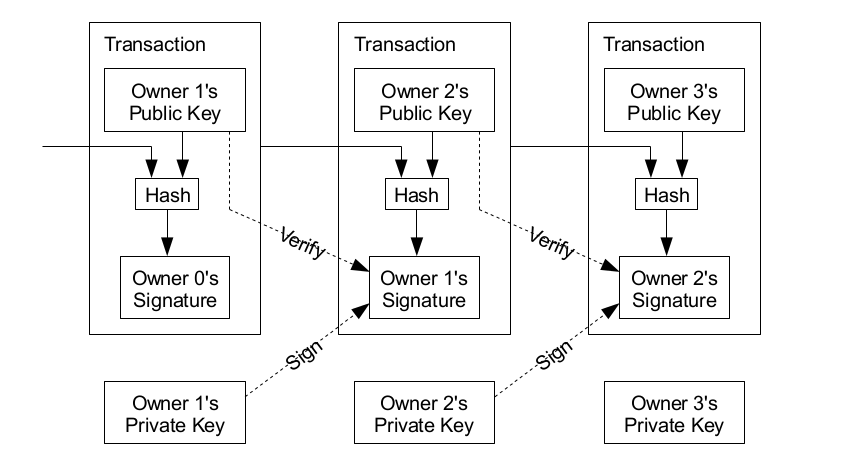
\includegraphics[width=0.8\textwidth]{images/coin.png}
   \caption{Modelo da moeda digital \cite{nakamoto2008bitcoin}.}
\end{figure}

\section*{Transações}

Uma transação inicia-se em poucos segundos e é confirmada geralmente em 10 minutos. Durante esse tempo a transação pode ser autenticada porém ainda reversível. As transações depois de confirmadas por grande parte dos nós honestos não podem ser revertidas, portanto é necessário confiar no futuro dono da moeda.

Para resolver o problema do gasto duplo o Bitcoin, as transações são publicamente anunciadas e são necessários participantes que concordem em uma história única da ordem em que são recebidas. O futuro dono precisa da prova que no momento da transação a maioria dos nós concordam que é o primeiro pagamento desta moeda do dono.

Para cifrar as transações o algoritmo utilizado é o  ECDSA, Assinatura Digital de Curvas Elípticas, assinando a alteração da propriedade possui as entradas: registros das transações antigas e a saída é um registro determinando o novo dono do Bitcoin, que será utilizado como entrada para futuras transações, abaixo um exemplo.

\begin{lstlisting}[Exemplo de uma transação Bitcoin com uma entrada e uma saída apenas]
Input:
Previous tx: f5d8ee39a430901c91a5917b9f2dc19d6d1a0e9cea205b009ca73dd04470b9a6
Index: 0
scriptSig: 304502206e21798a42fae0e854281abd38bacd1aeed3ee3738d9e1446618c4571d10
90db022100e2ac980643b0b82c0e88ffdfec6b64e3e6ba35e7ba5fdd7d5d6cc8d25c6b241501

Output:
Value: 5000000000
scriptPubKey: OP_DUP OP_HASH160 404371705fa9bd789a2fcd52d2c580b65d35549d
OP_EQUALVERIFY OP_CHECKSIG
\end{lstlisting}

A solução do Bitcoin utiliza um servidor de timestamp que funciona gerando um hash do bloco de itens e publica este hash. Cada timestamp inclue o timestamp anterior formando uma cadeia.

Para prevenir o problema de duplo gasto, o Bitcoin propõe um servidor timestamp duma rede distribuída peer-to-peer que gere um uma ordem cronológica das transações. O sistema é seguro enquanto os nós honestos coletivamente controlarem mais CPU power que um grupo de atacantes. A idéia é fomentar nodos que ajudem a validar as transações, não precisando de uma instituição que garanta que não haja duplo-pagamento.

Para implementar um servidor de timestamp distribuído é utilizado um sistema similar ao Hashcash, para proteger a rede e manter a rede decentralizada sem autoridade central. O trabalho requerido em média é exponencial ao número de bits zero. Uma vez que o trabalho satisfaz a prova de trabalho o bloco, a prova de trabalho é um voto por CPU.

Para compensar o aumento da velocidade de hardware durante o tempo, a dificuldade da \textit{proof-of-work}, prova de trabalho pode ser determinada alterando o número médio de blocos por hora. Os passos para executar a rede são:
\begin{itemize}
    \item Novas transações são comunicadas para todos os nós.
    \item Cada nó coleta novas transações para o bloco.
    \item Cada nó trabalha em encontrar a prova de trabalho de seu bloco.
    \item Quando um nó encontra um prova de trabalho, envia broadcast para todos os nodos.
    \item Nós aceitam o bloco apenas se todas as transações são validas e não foram gastos.
    \item Nós expressam a aceitação do bloco criando no próximo bloco da cadeia usando o hash de aceitação do bloco anterior.
\end{itemize}

Os nós sempre consideram a cadeia mais longa como correta no caso de dois nós fizeram broadcast simultâneo de diferentes versões do próximo bloco. Alguns podem receber uma ou outra primeiro, neste caso ele trabalha na primeira recebida porém salva a próxima caso a cadeira se torne maior. O broadcast necessita alcançar um número minimo de nós \cite{nakamoto2008bitcoin}.

Geralmente não são cobrado taxas para transações que envolvem Bitocoins, porém quando os valores são muito pequenos (menores que 0.01 XBT, ou 0.01 satoshis) ou muito novas elas não são gratuitas. Quando isto acontece a taxa recolhida é repassada aos nós que estão minerando, para incentivar a mantenção da rede.

Site para visualização em tempo real das transações que ocorrem \cite{realTime} na rede Bitcoin.

\section*{Legislação no Brasil}

Não existe legislação específica e decisões tomadas pelos tribunais limitam-se a casos de cartões de crédito ou transações bancárias na Internet. Se ambas as partes concordam que determinado produto ou serviço será pago por meio de Bitcoins e não em moeda corrente, trata-se de um contrato entre elas, com plena validade legal.

A conversão de Bitcoins em dinheiro real geralmente implica na utilização de corretores estrangeiros, cuja reputação ainda é desconhecida. Além disso os tribunais terão grande dificuldade em compreender o conceito de uma moeda criptográfica.

Uma questão essencial do Bitcoin, é a falta do lastro governamental, ou seja, a garantia para ser aceito no pagamento de dívidas. Para possuir valor real é necessário encontrar organizações dispostas a trocar BTCs por outras moedas, ou haver uma ampla gama de serviços e produtos à venda em Bitcoins como em \cite{trade}.

\section*{Geração de Bitcoins}
O número total de bitcoins aumenta num total pré-estabelecido até o limite de e cada vez o bloco é adicionado a cadeia. Estes novos bitcoins são dados para quem resolver o problema computacional da prova de trabalho. Para criar novas moedas é necessário que seja a primeira transação de um bloco.
\subsection*{Mineração}
O processo de mineração de Bitcoins serve para criar o registro de transações na rede e prover segurança. Inicialmente para ser executado em computadores pessoais.

Hoje é muito dificil minerar Bitcoins sozinho em casa, já que exitem dezenas de empresas e \textit{pools} que detem grande parte da rede, abaixo \ref{pools} o gráfico retirado de \cite{pools}. Além disso houveram muitos avanços na construção de hardwares especializados para mineração.

\begin{figure}[H]
   \label{pools}
   \centering
   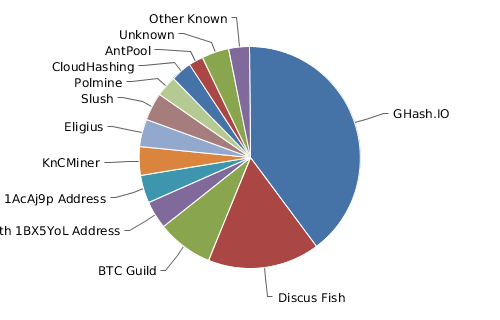
\includegraphics[width=0.8\textwidth]{images/pools.png}
   \caption{Hashrate distribution retirado de \cite{pools}.}
\end{figure}

O sistema reajusta o nível de dificuldade de criptografia de acordo com o processamento coletivo da rede, portanto, quanto mais perto chegar desse número, mais difícil será conseguir BTC na mineração virtual.

Abaixo a tabela \ref{compare} comparação de velocidade e entre computadores pessoais, GPUS, FPGAS e ASIC para calcular hashs. O calculo utilizou com base a dificuldade atual que é de 16818461371.1610 e 25 bitcoins por bloco.

\begin{table}[!ht]
\centering
\label{compare}
\scriptsize
\begin{tabular}{|c|c|c|}
\hline
\textbf{HW} & \textbf{Mhash/s} & \textbf{Days to gerenate one block} \\ \hline
CPU Pentium III & 0.39 & 2200132235.6 \\ \hline
CPU Core i7 3930k & 66.6 & 12553307.0 \\ \hline
GPU ATI 5850 & 432.15 & 1934629.8 \\ \hline
GPU NVidia Tesla S2070 & 749.23 & 1115879.3 \\ \hline
FPGA BitForce SHA256 Single & 832 & 1004868.1 \\ \hline
GPU 6 x ATI 5850 & 2135 & 391592.6 \\ \hline
FPGA KnCMiner Mars & 6000 & 139341.7 \\ \hline
ASIC Avalon2 & 300000 & 27868.3 \\ \hline
ASIC Minerscube & 15000000 & 55.7 \\ \hline  
\end{tabular}
\end{table}

\section*{Monetização e comércio}

Existem serviços de câmbio do Bitcoin para diversas moedas inclusive para outras \textit{crypto-currences}.

O \cite{trade} possui uma extensa lista dos bens de consumo possíveis de serem comprados por Bitcoins.

\section*{Carteira Digital}
A carteira é um arquivo na qual contem uma coleção de chaves privadas. Ao entrar na comunidade monetária, seus ganhos serão armazenados em uma carteira virtual, um  número arbitrário de chaves que vão identificar suas transações. A responsabilidade de guardar a carteira é do usuário, existem diversos serviços para armazenamento remoto, como o Blockchain.

Existe um formato chamado WIF, Wallet Import Format, que é uma forma de codificar uma chave privada ECDSA de forma mais fácil para copiar \cite{wif}. 

Existe também iniciativas para armazenamento em hardware com Pi Wallet, TREZOR e BitcoinCard entre outros disponiveis em \cite{hardWallet}

\section{Ferramentas de Mineração e Carteira Digital}

Existem diversos serviços de armazenamento de sua carteira digital, um dos mais conhecidos e recomendado inicialmente é o Blockchain. A mesma carteira pode ser acessada utilizando o Blockchain para celular Android ou IOS, dispõe de diversos recursos de segurança, como notificação via sms, autenticação de dois passos, etc.

Formas mais interessantes de se adquirir Bitcoin é através de serviços e doações. Existe um plugin para WordPress que torna possível aceitar doações de bitcoin direto para sua carteira digital. http://bestbitcoin.com.br/plugin-bitcoin-donations/

Atualmente é muito difícil de minerar Bitcoins, sozinho é praticamente impossível, é necessário participar de pools de mineração. Um bastante conhecido é o pool http://mining.bitcoin.cz/. Na qual fiz cadastro e foi criado um \textit{pool worker}.

A ferramenta local utilizada foi o https://github.com/m0mchil/poclbm.git /


\section*{Problemas}
Utilizando como base \cite{hardProblems}, os principais problemas do Bitcoin são:

\begin{description}
\item[Espaço de armazenamento:] todos os nós precisam armazenar todas as transações.
\item[Centralização da mineração:] monopolização da rede de grandes pools \cite{pools}.
\item[Gasto inútil de energia:] a prova de trabalho do Bitcoin é inútil, já que encontrar uma sequencia de zero bits no início de um hash não é utilizado para nada. 

\item[Instabilidade no valor:] Bitcoin reduz o suprimento exponencialmente, a demanda é volátil mas o suprimento é pré-determinado, isto faz com que o valor flutue demais, podendo trazer perdas em negociações.
\end{description}

\section*{Benefícios}
\begin{description}
\item[Aberta:] pode ser útil para pessoas em países totalitários que precisam de privacidade, por exemplo. 
\item[Redução de custos:] não existe uma Instituição, como um banco, pois a responsabilidade de manter a carteira é do próprio usuário e a validação e feita pela rede.
\item[Microtransações:] geralmente não é cobrado um valor na transação podendo ser utilizado valores mínimos para diversos serviços, habilitadas através da redução de custos.
\end{description}

\section*{Presente}
O atual valor de mercado do Bitcoin medido em dólares americanos é 8,058,733,725.
A Microsoft publicou \cite{bing} através do Bing uma ferramenta para conversão automática de valores de Bitcoin para outras moedas. Já existe uma casa de câmbio em funcionamento no Brasil, foi inaugurada em Curitiba e faz troca em diversas moedas. 

\section*{Futuro}

Moedas baseadas no Bitcoin porém utilizando diferentes algoritmos para validar as transações, além de estratégias para minimizar os problemas já reconhecidos do Bitcoin. Um exemplo é a moeda Primecoin que utilização da prova de trabalho baseada em econtrar sequências de números primos.

O New Economic Moviment \cite{nem}, propõe uma moeda aonde a validação do trabalho utiliza um conceito de \textit{proof-of-excelence} aonde pessoas pessoas ricas ou que adotaram a tecnologia antes não tem vantagens em adquirir moedas, mas quem realmente executa uma tarefa que beneficia a comunidade.


\bibliography{relatorio}{}
\bibliographystyle{plain}

\end{document}
